\documentclass[tikz,border=3pt]{standalone}
% Shared preamble for the standalone TikZ diagrams (included after \documentclass).
% Build with build.sh. Language is selected with \def\VI{1} (Vietnamese) or by default English:
%   \LL{English text}{Văn bản tiếng Việt}
\usepackage{fontspec}
\IfFontExistsTF{Times New Roman}{\setmainfont{Times New Roman}}{%
  \setmainfont{times.ttf}[Path=/mnt/c/Windows/Fonts/,
    BoldFont=timesbd.ttf,ItalicFont=timesi.ttf,BoldItalicFont=timesbi.ttf]}
\usepackage{xcolor}
\usepackage{tikz}
\usetikzlibrary{arrows.meta,positioning,calc,fit,backgrounds,patterns,shapes.misc,decorations.pathreplacing}

\newcommand{\LL}[2]{\ifdefined\VI #2\else #1\fi}
\hyphenpenalty=10000 \exhyphenpenalty=10000 \tolerance=9999 \emergencystretch=3em

% --- palette (print-safe: meaning is never carried by colour alone) -----------
\definecolor{ink}{HTML}{1F2937}
\definecolor{muted}{HTML}{6B7280}
\definecolor{rule}{HTML}{9CA3AF}
\definecolor{shfill}{HTML}{DCE8F5}   % shared
\definecolor{shline}{HTML}{2F5D8C}
\definecolor{dedfill}{HTML}{FBE5CF}  % dedicated
\definecolor{dedline}{HTML}{B5651D}
\definecolor{neutral}{HTML}{F3F4F6}
\definecolor{appfill}{HTML}{F6F9FC}
\definecolor{appline}{HTML}{7C93AD}
\definecolor{ctlfill}{HTML}{EFEAF7}
\definecolor{ctlline}{HTML}{6B5B95}
\definecolor{warn}{HTML}{B91C1C}
\definecolor{ta}{HTML}{2A9D8F}       % tenant A
\definecolor{tb}{HTML}{E09F3E}       % tenant B
\definecolor{tc}{HTML}{8E6BBF}       % tenant C
\colorlet{taL}{ta!22}
\colorlet{tbL}{tb!28}
\colorlet{tcL}{tc!24}

\tikzset{
  >=Latex,
  every node/.style={font=\footnotesize, text=ink, inner sep=2pt},
  box/.style={draw=ink!65, rounded corners=1.6pt, line width=0.5pt, fill=white,
              align=center, inner sep=3pt, minimum height=5mm},
  shared/.style={box, fill=shfill, draw=shline},
  ded/.style={box, fill=dedfill, draw=dedline},
  plain/.style={box, fill=neutral, draw=rule},
  ta/.style={box, fill=taL, draw=ta},
  tb/.style={box, fill=tbL, draw=tb},
  tc/.style={box, fill=tcL, draw=tc},
  tenantA/.style={ta}, tenantB/.style={tb}, tenantC/.style={tc},
  zone/.style={draw=appline, fill=appfill, rounded corners=2.5pt, line width=0.6pt},
  ctlzone/.style={draw=ctlline, fill=ctlfill, rounded corners=2.5pt, line width=0.6pt},
  ttl/.style={font=\small\bfseries, text=ink, align=left, inner sep=1pt},
  cp/.style={font=\scriptsize, text=muted, align=center, inner sep=1pt},
  note/.style={font=\scriptsize, text=muted, align=left, inner sep=1pt},
  arr/.style={->, line width=0.6pt, draw=ink!80},
  arrm/.style={->, line width=0.6pt, draw=muted, dashed},
  link/.style={line width=0.5pt, draw=muted},
  bound/.style={line width=0.8pt, draw=warn, dash pattern=on 3pt off 2pt},
  badge/.style={circle, fill=ink, text=white, font=\scriptsize\bfseries, inner sep=1.2pt, minimum size=3.6mm},
}

% a small user glyph (head + shoulders) centred at the given coordinate, colour as 3rd arg

% user glyph: head and shoulders, centred at (x,y); 3rd argument = colour
\newcommand{\user}[3]{%
  \fill[#3] (#1,#2) circle (0.85mm);
  \fill[#3] ($(#1,#2)+(-1.5mm,-2.5mm)$) arc (180:0:1.5mm) -- cycle;}

% Figure: multi-user vs multi-instance vs multi-tenant, drawn with one visual vocabulary.
\begin{document}
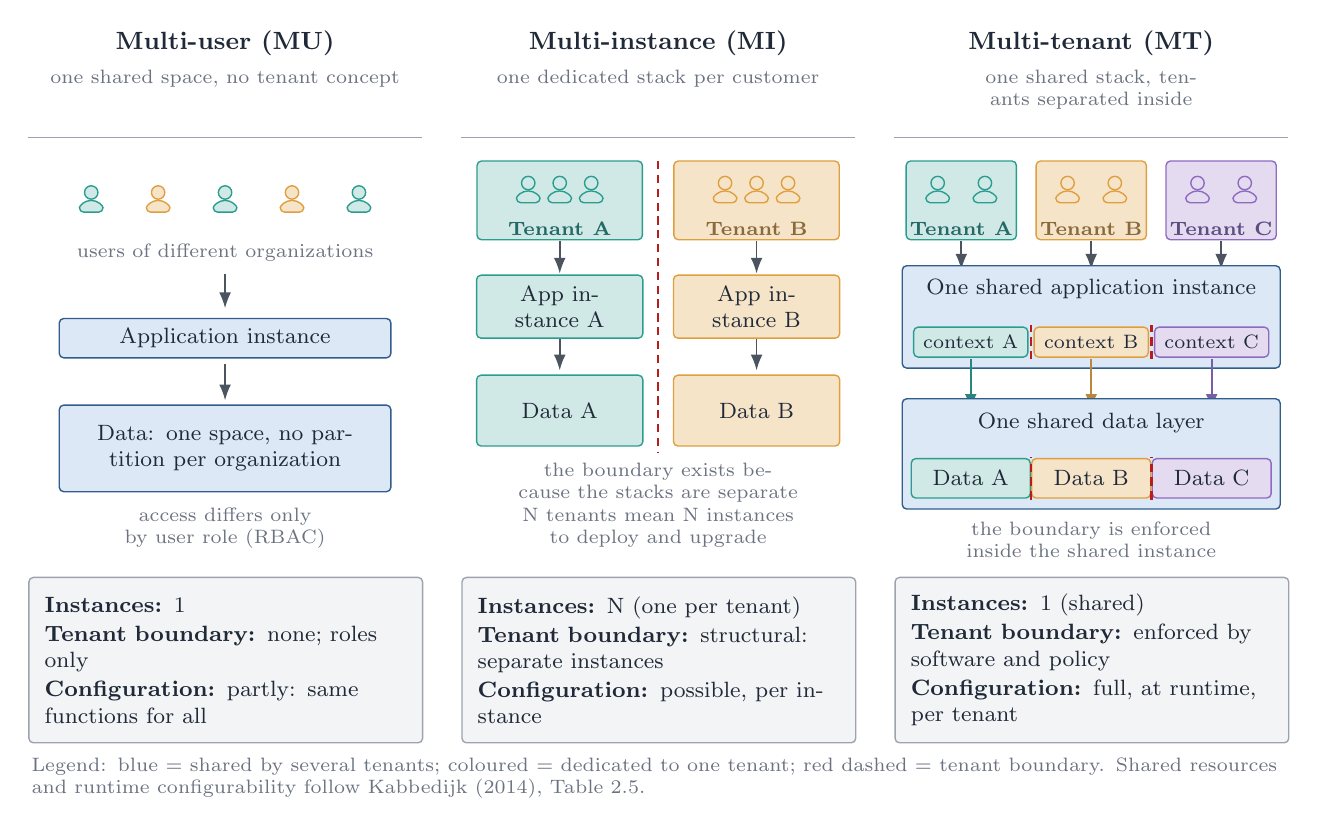
\begin{tikzpicture}[x=1mm,y=1mm]

% ---------------------------------------------------------------- panel titles
\foreach \x/\en/\vi/\sen/\svi in {
  0/{Multi-user (MU)}/{Đa người dùng (MU)}/{one shared space, no tenant concept}/{một không gian chung, không có khái niệm thuê bao},
  55/{Multi-instance (MI)}/{Đa thể hiện (MI)}/{one dedicated stack per customer}/{mỗi khách hàng một bộ riêng},
  110/{Multi-tenant (MT)}/{Đa thuê bao (MT)}/{one shared stack, tenants separated inside}/{một bộ dùng chung, các thuê bao được tách biệt bên trong}} {
  \node[ttl] at (\x+25,94) {\LL{\en}{\vi}};
  \node[cp,text width=48mm,anchor=north] at (\x+25,91) {\LL{\sen}{\svi}};
  \draw[rule,line width=0.4pt] (\x,82) -- (\x+50,82);
}

% ================================================================= MU panel
\begin{scope}[shift={(0,0)}]
  \foreach \i/\c in {0/ta,1/tb,2/ta,3/tb,4/ta} { \user{8+\i*8.5}{75}{\c} }
  \node[cp,text width=48mm] at (25,67.4) {\LL{users of different organizations}{người dùng thuộc nhiều tổ chức}};
  \draw[arr] (25,64.6) -- (25,60.3);
  \node[shared,minimum width=42mm,text width=40mm] (muapp) at (25,56.5) {\LL{Application instance}{Thể hiện ứng dụng}};
  \draw[arr] (25,53.2) -- (25,48.6);
  \node[shared,minimum width=42mm,minimum height=11mm,text width=40mm] (mudata) at (25,42.5) {\LL{Data: one space, no partition per organization}{Dữ liệu: một không gian, không phân vùng theo tổ chức}};
  \node[cp,text width=46mm] at (25,32.4) {\LL{access differs only by user role (RBAC)}{khác biệt chỉ ở vai trò người dùng (RBAC)}};
\end{scope}

% ================================================================= MI panel
\begin{scope}[shift={(55,0)}]
  \foreach \cx/\c/\n/\nv in {12.5/ta/A/A, 37.5/tb/B/B} {
    \node[\c,minimum width=21mm,minimum height=10mm] at (\cx,74) {};
    \user{\cx-4}{76.2}{\c}  \user{\cx}{76.2}{\c}  \user{\cx+4}{76.2}{\c}
    \node[font=\scriptsize\bfseries,text=\c!55!ink] at (\cx,70.4) {\LL{Tenant \n}{Thuê bao \nv}};
    \draw[arr] (\cx,68.9) -- (\cx,64.7);
    \node[\c,minimum width=21mm,minimum height=8mm,text width=19mm] at (\cx,60.5) {\LL{App instance \n}{Thể hiện ứng dụng \nv}};
    \draw[arr] (\cx,56.4) -- (\cx,52.4);
    \node[\c,minimum width=21mm,minimum height=9mm,text width=19mm] at (\cx,47.3) {\LL{Data \n}{Dữ liệu \nv}};
  }
  \draw[bound] (25,79) -- (25,42);
  \node[cp,text width=48mm] at (25,38.2) {\LL{the boundary exists because the stacks are separate}{ranh giới tồn tại vì các bộ thể hiện tách rời}};
  \node[cp,text width=48mm] at (25,32.4) {\LL{N tenants mean N instances to deploy and upgrade}{N thuê bao nghĩa là N thể hiện cần triển khai và nâng cấp}};
\end{scope}

% ================================================================= MT panel
\begin{scope}[shift={(110,0)}]
  \foreach \x/\c/\n in {8.5/ta/A, 25/tb/B, 41.5/tc/C} {
    \node[\c,minimum width=14mm,minimum height=10mm] at (\x,74) {};
    \user{\x-3}{76.2}{\c}  \user{\x+3}{76.2}{\c}
    \node[font=\scriptsize\bfseries,text=\c!55!ink] at (\x,70.4) {\LL{Tenant \n}{Thuê bao \n}};
    \draw[arr] (\x,68.9) -- (\x,65.2);
  }
  \node[shared,minimum width=48mm,minimum height=13mm] (mtapp) at (25,59.2) {};
  \node[font=\footnotesize,text width=46mm,align=center] at (25,62.7) {\LL{One shared application instance}{Một thể hiện ứng dụng dùng chung}};
  \node[ta,minimum width=14.5mm,minimum height=3.8mm,font=\scriptsize] at (9.7,56) {\LL{context A}{ngữ cảnh A}};
  \node[tb,minimum width=14.5mm,minimum height=3.8mm,font=\scriptsize] at (25,56) {\LL{context B}{ngữ cảnh B}};
  \node[tc,minimum width=14.5mm,minimum height=3.8mm,font=\scriptsize] at (40.3,56) {\LL{context C}{ngữ cảnh C}};
  % routing by tenant context
  \foreach \x/\c in {9.7/ta, 25/tb, 40.3/tc} { \draw[->,line width=0.6pt,draw=\c!80!ink] (\x,53.9) -- (\x,47.4); }
  \node[shared,minimum width=48mm,minimum height=14mm] (mtdata) at (25,41.8) {};
  \node[font=\footnotesize,text width=46mm,align=center] at (25,45.7) {\LL{One shared data layer}{Một tầng dữ liệu dùng chung}};
  \node[ta,minimum width=14.5mm,minimum height=5mm,text width=13mm] at (9.7,38.7) {\LL{Data A}{Dữ liệu A}};
  \node[tb,minimum width=14.5mm,minimum height=5mm,text width=13mm] at (25,38.7) {\LL{Data B}{Dữ liệu B}};
  \node[tc,minimum width=14.5mm,minimum height=5mm,text width=13mm] at (40.3,38.7) {\LL{Data C}{Dữ liệu C}};
  \draw[bound] (17.35,36) -- (17.35,41.4);
  \draw[bound] (32.65,36) -- (32.65,41.4);
  \draw[bound] (17.35,53.8) -- (17.35,58.2);
  \draw[bound] (32.65,53.8) -- (32.65,58.2);
  \node[cp,text width=48mm,anchor=north] at (25,33.6) {\LL{the boundary is enforced inside the shared instance}{ranh giới được thực thi bên trong thể hiện dùng chung}};
\end{scope}

% ---------------------------------------------------------------- property strips
\foreach \x/\ia/\iv/\ba/\bv/\ca/\cv in {
  0/{1}/{1}/{none; roles only}/{không có; chỉ có vai trò}/{partly: same functions for all}/{một phần: cùng chức năng cho mọi người},
  55/{N (one per tenant)}/{N (mỗi thuê bao một)}/{structural: separate instances}/{cấu trúc: các thể hiện riêng}/{possible, per instance}/{có thể, theo từng thể hiện},
  110/{1 (shared)}/{1 (dùng chung)}/{enforced by software and policy}/{do phần mềm và chính sách thực thi}/{full, at runtime, per tenant}/{đầy đủ, lúc chạy, theo thuê bao}} {
  \node[box,fill=neutral,draw=rule,minimum width=50mm,minimum height=21mm,anchor=north west,align=left,text width=46mm,inner sep=3pt]
    at (\x,26.2) {%
    \textbf{\LL{Instances:}{Số thể hiện:}} \LL{\ia}{\iv}\\[1pt]
    \textbf{\LL{Tenant boundary:}{Ranh giới thuê bao:}} \LL{\ba}{\bv}\\[1pt]
    \textbf{\LL{Configuration:}{Cấu hình:}} \LL{\ca}{\cv}};
}
\node[note,anchor=north west,text width=160mm] at (0,3.6) {\LL{Legend: blue = shared by several tenants; coloured = dedicated to one tenant; red dashed = tenant boundary. Shared resources and runtime configurability follow Kabbedijk (2014), Table 2.5.}{Chú giải: xanh dương = dùng chung cho nhiều thuê bao; màu riêng = dành cho một thuê bao; đứt nét đỏ = ranh giới thuê bao. Việc dùng chung tài nguyên và khả năng cấu hình lúc chạy theo Kabbedijk (2014), Bảng 2.5.}};

\end{tikzpicture}
\end{document}
